\documentclass[10pt,a4paper]{article}
\usepackage[utf8]{inputenc}
\usepackage[margin=1.5cm]{geometry}
\usepackage{titlesec}
\usepackage{enumitem}
\usepackage{xcolor}
\usepackage{hyperref}
\usepackage{graphicx}

\definecolor{primary}{RGB}{30, 41, 59}
\definecolor{accent}{RGB}{37, 99, 235}
\definecolor{text}{RGB}{51, 65, 85}

\hypersetup{
  colorlinks=true,
  urlcolor=accent,
  linkcolor=accent
}

\titleformat{\section}{\large\bfseries\color{primary}}{}{0em}{}[\vspace{-2pt}\rule{\textwidth}{0.8pt}]
\titlespacing{\section}{0pt}{8pt}{4pt}

\setlist[itemize]{leftmargin=1.2em, itemsep=1.5pt, topsep=1.5pt, parsep=0pt}

\newcommand{\role}[4]{
  \vspace{2pt}
  \noindent\textbf{#1} \hfill \textit{#2} \\
  \textit{\color{text}#3} \hfill \textit{\color{text}#4}
  \vspace{1pt}
}

\begin{document}
\pagestyle{empty}

% ================= HEADER =================
\begin{minipage}[c]{0.80\textwidth}
  {\Huge\bfseries Prabhavit Gupta}\\[3pt]
  {\color{accent}\large AI Automation Engineer: Low-Code Workflows, LLM Pipelines \& Media Automation}\\[6pt]
  {\footnotesize +39 351 610 7807 ~$\vert$~
  \href{mailto:prabhavitg@gmail.com}{prabhavitg@gmail.com} ~$\vert$~
  \href{https://www.linkedin.com/in/prabhavit/}{linkedin.com/in/prabhavit} ~$\vert$~
  \href{https://github.com/prab-gupta}{github.com/prab-gupta} ~$\vert$~
  Venice, Italy}
\end{minipage}\hfill
\begin{minipage}[c]{0.18\textwidth}
  \raggedleft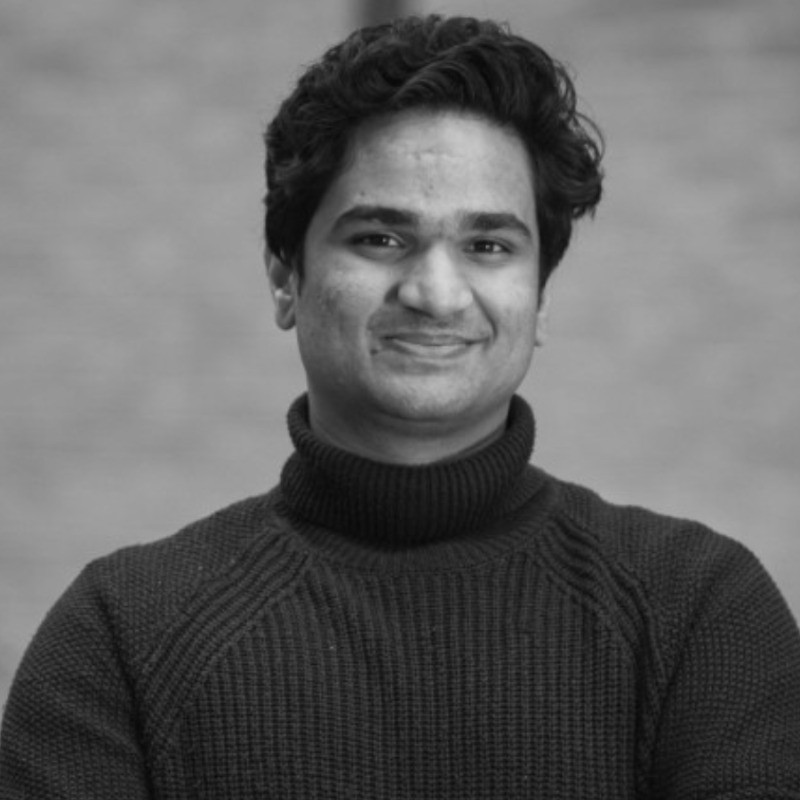
\includegraphics[width=2.0cm]{photo.jpg}
\end{minipage}
\vspace{-2pt}

% ================= SUMMARY =================
\section{Summary}
AI Automation Engineer with 3 years of hands-on experience designing, shipping, and evaluating production LLM agents, automated creative/media workflows, and resilient integration pipelines. At FlowSpace, architected multi-step autonomous workflows utilizing live REST API function calling, built automated data ingestion and asset processing pipelines with Airtable and Supabase schemas, and integrated low-code automation platforms (n8n, Make) to orchestrate complex third-party services. Strong expertise in Node.js/JavaScript, RESTful APIs, LLM tool calling (OpenAI, Claude), prompt engineering, and automated testing with Playwright. Based in Venice, Italy with EU Long Term Residence Permit (unrestricted EU work authorization without sponsorship). Immediately available.

% ================= TECHNICAL EXPERTISE =================
\section{Technical Expertise}
\begin{itemize}
  \item \textbf{Low-Code \& Workflow Automation:} n8n, Make, Airtable, Zapier, Webhook listeners, Idempotent event processing, Event-driven architecture, Cron schedulers, Error alerting.
  \item \textbf{AI Systems \& LLM Integration:} OpenAI API, Anthropic Claude API, Structured JSON output schemas, Prompt engineering, AI Agents, Tool calling, Media/asset generation workflows.
  \item \textbf{Software Development:} JavaScript (Node.js), TypeScript, RESTful API architecture, Playwright, Supabase, PostgreSQL, Laravel, Docker, Git/GitHub.
  \item \textbf{Platforms \& Integrations:} Airtable scripting, Meta/AppLovin API concepts, Cloud asset storage, Automated regression testing, Postman.
  \item \textbf{Languages \& Authorization:} Hindi (Native), English (C1 Professional), Italian (Beginner). European Long Term Residence Permit (No EU sponsorship required).
\end{itemize}

% ================= EXPERIENCE =================
\section{Experience}

\role{\href{https://flowspace.co}{FlowSpace.co}}{Mar 2024 - Aug 2026}{Lead Developer (Full-time, Freelance)}{London, UK (remote)}
\begin{itemize}
  \item Architected and deployed production customer support AI agents using LLM tool calling and live REST API function calling to query platform availability and execute bookings, with confidence thresholds and fallback routing.
  \item Built an automated knowledge ingestion and listing bot with human-in-the-loop review: parsed heterogeneous documents (PDFs, spreadsheets, web pages) into structured database records using LLM extraction prompts, creating 900+ verified listings.
  \item Engineered agentic developer workflows and tooling using Claude Code, TypeScript, and automated testing, accelerating feature delivery cycles across the engineering team.
  \item Directed platform architecture migration off a legacy stack to a modern Next.js, TypeScript, and Laravel backend, establishing reliable schema contracts and API specifications.
  \item Integrated external REST APIs (OfficeRnD, Nexudus, Stripe) with idempotent event handling and automated webhook reconciliation.
  \item Implemented token tracking, prompt versioning, and end-to-end regression testing with Playwright to maintain high output fidelity across production agent runs.
  \item Scaled platform user base from 2,000 to 4,500+ active users through iterative product engineering and resilient backend automations.
\end{itemize}

\role{Urlink}{Apr 2025 - Jul 2025}{Project Manager \& AI Assisted Developer (Freelance)}{Barcelona, Spain (remote)}
\begin{itemize}
  \item Led technical delivery of AI-assisted web applications, coordinating API contracts, database schemas, and external integrations.
  \item Evaluated commercial LLM APIs (OpenAI, Anthropic) across task types, optimizing prompt structures and model selection for latency and output consistency.
  \item Implemented automated CI/CD checks and test suites, ensuring clean code releases and minimal deployment regressions.
\end{itemize}

\role{Independent Technical Consultant}{Aug 2023 - Feb 2024}{AI Solutions \& Automation Engineer}{Venice, Italy}
\begin{itemize}
  \item Developed custom AI automations, agent prototypes, and data extraction pipelines for European SME clients using n8n, Playwright, and LLM APIs.
  \item Implemented idempotent webhook listeners and CRM data synchronization flows, replacing error-prone manual administrative processes.
  \item Built automated verification scripts with Playwright and Postman for regression testing and continuous data validation.
\end{itemize}

% ================= EDUCATION =================
\section{Education}

\role{Ca' Foscari University of Venice}{2020 - 2024}{BA in Philosophy, International and Economic Studies}{Venice, Italy}
\begin{itemize}
  \item Rigorous focus on formal logic, statistical reasoning, decision theory, and analytical problem-solving applied directly to software systems and algorithmic workflows.
\end{itemize}

\end{document}
